% ANDER MARTINEZ 2014

\documentclass{article}
\usepackage{url}
\usepackage{hyperref}
\usepackage{graphicx}
\usepackage[margin=1in]{geometry}

\title{gamelad -- a gameboy emulator for STM32F4}
\author{Ander Martinez}
\date{\today}

\begin{document}
\maketitle

\section{Introduction}
My intention intention with this project was to understand better
how computer hardware works. That's the reason why I chose to  
emulate a simple hardware such as GameBoy.

The original GameBoy has custom CPU based on the Intel 8080 with
the instruction set borrowed from the Zilog Z80. The chip's official
name is Sharp LR35902 and it's clocked at 4MHz.

The GB also has: a screen resolution of $160 \times 144$
($20 \times 18$ tiles) and four colours (grayscale);
0xFFFF memory space with adressable registers and lots of memory
magic; an interrupt system; timers and different memory bank controllers
which allowed for additional hardware on cartridges. Only MBC1 cartridge
emulation was attempted (maximum of 2MB ROM and 32KB of RAM).

\section{Gamepad}
A six-button Sega Genesis/Mega Drive controller was used.
Which has four directions, a start button and six game buttons
(A,B,C,X,Y,Z).
As the original GameBoy had only two game buttons (A and B) and
START and SELECT buttons besides the four directions technically
a 3 button controller could have also been used and the coding
should work the same for this kind of controller. The only
reason I had to use the 6-button version is because nowadays it's
more afordable (\$5.22 USD at amazon).
The top three buttons (X, Y and Z) are not being used, because
they are unnecessary for gameboy emulation.

\begin{table}[!h]
  \centering
  \begin{tabular}{|l|r|}
    \hline
    GENESIS & GAMEBOY \\
    \hline
    directions & directions \\
    START & START \\
    A & B \\
    B & A \\
    C & SELECT \\
    \hline
  \end{tabular}
  \caption{Button equivalences.}
\end{table}

The gamepad has been wired to the board as shown in the table \autoref{tab:wires}.


\begin{table}[!h]
  \centering
  \begin{tabular}{|l|c|c|c|r|}
    \hline
    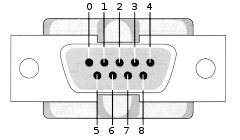
\includegraphics[scale=.5]{gamepad_pins.png}
    & Description & STM32F4-BB PIN & name & STM32F4 GPIO \\
    \hline
    0 & $V_{cc}$      & 40 & +3V        & -        \\
    1 & RIGHT         & 28 & GPIO6      & GPIOA 10 \\
    2 & LEFT          & 18 & GPIO2      & GPIOA 5  \\
    3 & DOWN          & 24 & GPIO4      & GPIOA 8  \\
    4 & UP            & 16 & GPIO1      & GPIOD 11 \\
    5 & START/C       & 5  & UART1\_TXD & GPIOB 6  \\
    6 & GND           & 10 & GND        & -        \\
    7 & Select Signal & 22 & GPIO3      & GPIOA 15 \\
    8 & A/B           & 26 & GPIO5      & GPIOA 3  \\
    \hline
  \end{tabular}
  \caption{Button equivalences.}
  \label{tab:wires}
\end{table}

\begin{thebibliography}{9}
  \bibitem{GBCPUman.pdf}
    Game Boy \texttrademark CPU Manual.
    \url{http://marc.rawer.de/Gameboy/Docs/GBCPUman.pdf}
  \bibitem{GameBoyProgrammingManual.pdf}
    GAME BOY programming manual.
    \url{http://students.washington.edu/fidelp/galp/megaguides/GameBoyProgrammingManual.pdf}
  \bibitem{gbspec.txt} 
    Everything You Always Wanted To Know About GAMEBOY.
    \url{http://www.devrs.com/gb/files/gbspec.txt}
  \bibitem{segasix.txt}
    Sega Six Button Controller Hardware Info
    \url{http://www.cs.cmu.edu/~chuck/infopg/segasix.txt}
  \bibitem{STM32F4DIS-BB User Manual.pdf}
    STM32F4DIS-BB User Manual
\end{thebibliography}
\end{document}

